%
\documentclass[12pt]{article}

% The usual packages
\usepackage{booktabs}
\usepackage{array}
\usepackage{subcaption}

\usepackage{fullpage}
\usepackage{breakcites}
\usepackage{setspace}
\usepackage{endnotes}
\usepackage{mathtools} % for \mathclap
%\usepackage{float} % can't use with floatrow
\usepackage{amsmath}
\usepackage{amsfonts}
\usepackage{amssymb}
\usepackage{rotating}
\usepackage{longtable}
\usepackage{microtype}
\usepackage{graphicx}
\usepackage{hyperref}
%\usepackage[usenames,dvipsnames]{color}
\usepackage{url}
\usepackage{natbib}
\usepackage{framed}
\usepackage{epigraph}
\usepackage{lipsum}
\usepackage{textcomp} % for \textrightarrow
\usepackage{dcolumn}
\usepackage{nameref}
\usepackage{booktabs}
\usepackage{float}
%\restylefloat{table}
\bibpunct{(}{)}{;}{a}{}{,}

% kable packages
\usepackage{booktabs}
\usepackage{longtable}
\usepackage{array}
\usepackage{multirow}
\usepackage[table]{xcolor}
\usepackage{wrapfig}
\usepackage{float}
\usepackage{colortbl}
\usepackage{pdflscape}
\usepackage{tabu}
\usepackage{threeparttable}
\usepackage{threeparttablex}
\usepackage[normalem]{ulem}
\usepackage{makecell}

% Set paragraph spacing the way I like
\parskip=0pt
\parindent=20pt

%\usepackage{helvet}
%\usepackage[labelfont={bf}, margin=0cm, font=small, skip=0pt]{caption}

\newcommand\numberthis{\addtocounter{equation}{1}\tag{\theequation}}

% Define mathematical results
\newtheorem{lemma}{Lemma}
\newtheorem{proposition}{Proposition}
\newtheorem{theorem}{Theorem}
\newtheorem{claim}{Claim}
\newenvironment{proof}[1][Proof]{\begin{trivlist}
\item[\hskip \labelsep {\bfseries #1}]}{\end{trivlist}}
\newenvironment{definition}[1][Definition]{\begin{trivlist}
\item[\hskip \labelsep {\bfseries #1}]}{\end{trivlist}}
\newenvironment{example}[1][Example]{\begin{trivlist}
\item[\hskip \labelsep {\bfseries #1}]}{\end{trivlist}}
\newenvironment{remark}[1][Remark]{\begin{trivlist}
\item[\hskip \labelsep {\bfseries #1}]}{\end{trivlist}}
\DeclareMathOperator*{\argmin}{arg\,min}
\DeclareMathOperator{\med}{med}
\DeclareMathOperator*{\E}{\text{E}}
%\DeclareMathOperator*{\Pr}{\text{Pr}}

%Set up fonts the way I like
%\usepackage{tgpagella}
%\usepackage[T1]{fontenc}
%\usepackage[bitstream-charter]{mathdesign}

%% Baskervald
%\usepackage[lf]{Baskervaldx} % lining figures
%\usepackage[bigdelims,vvarbb]{newtxmath} % math italic letters from Nimbus Roman
%\usepackage[cal=boondoxo]{mathalfa} % mathcal from STIX, unslanted a bit
%\renewcommand*\oldstylenums[1]{\textosf{#1}}

%\usepackage[T1]{fontenc}
%\usepackage{newtxtext,newtxmath}

% A special command to create line break in table cells
\newcommand{\specialcell}[2][c]{%
 \begin{tabular}[#1]{@{}c@{}}#2\end{tabular}}

%% Set up lists the way I like
% Redefine the first level
\renewcommand{\theenumi}{\arabic{enumi}.}
\renewcommand{\labelenumi}{\theenumi}
% Redefine the second level
\renewcommand{\theenumii}{\alph{enumii}.}
\renewcommand{\labelenumii}{\theenumii}
% Redefine the third level
\renewcommand{\theenumiii}{\roman{enumiii}.}
\renewcommand{\labelenumiii}{\theenumiii}
% Redefine the fourth level
\renewcommand{\theenumiv}{\Alph{enumiv}.}
\renewcommand{\labelenumiv}{\theenumiv}
% Eliminate spacing around lists
\usepackage{enumitem}
\setlist{nolistsep}

% Create footnote command so that my name
% has an asterisk rather than a one.
\long\def\symbolfootnote[#1]#2{\begingroup%
\def\thefootnote{\fnsymbol{footnote}}\footnote[#1]{#2}\endgroup}
%\usepackage{footmisc}
%\renewcommand{\thefootnote}{\symbolfootnote{footnote}}

% Create the colors I want
\usepackage{color, xcolor}
\definecolor{color1}{RGB}{217,95,2}  % orange
\definecolor{color2}{RGB}{27,158,119}  % green
\definecolor{color3}{RGB}{117,112,179}  % purple

% for colored \left( and \right)
\newcommand{\cleft}[2][.]{%
  \begingroup\colorlet{savedleftcolor}{.}%
  \color{#1}\left#2\color{savedleftcolor}%
}
\newcommand{\cright}[2][.]{%
  \color{#1}\right#2\endgroup
}

% for drawing arrows
\usepackage{tikz}
\usetikzlibrary{calc,shapes}

\newcommand{\tikzmark}[1]{\tikz[overlay,remember picture] \node (#1) {};}
\newcommand{\DrawBox}[2]{%
  \begin{tikzpicture}[overlay,remember picture]
    \draw[->,shorten >= 6pt, shorten <= 2pt, out=-90, in=85, distance=1.3cm, color2, thick] (MarkA.east) to (MarkB.east);
    \draw[->,shorten >= 6pt, shorten <= 2pt, out=-90, in=90, distance=1cm, color2, thick] (MarkC.west) to (MarkD.east);
  \end{tikzpicture}
}

% remarks by equations
\newcommand{\justif}[2]{&{#1}&\text{#2}}


% set up pdf
\hypersetup{
pdftitle={}, % title
pdfauthor={Carlisle Rainey}, % author
pdfkeywords={bias} {first difference} {marginal effect} {quantities of interest} {maximum likelihood}
pdfnewwindow=true, % links in new window
colorlinks=true, % false: boxed links; true: colored links
linkcolor=black, % color of internal links
citecolor=black, % color of links to bibliography
filecolor=blue, % color of file links
urlcolor=blue % color of external links
}

% section headers
%\usepackage[scaled]{helvet}
%\renewcommand\familydefault{\sfdefault}
%\usepackage[T1]{fontenc}
%\usepackage{titlesec}
%\titleformat{\section}
%  {\normalfont\sffamily\Large\bfseries}
%  {\thesection}{1em}{}
%\titleformat{\subsection}
%  {\normalfont\sffamily\large\bfseries}
%  {\thesection}{1em}{}
%  \titleformat{\subsubsection}
%  {\normalfont\sffamily\bfseries}
%  {\thesection}{1em}{}

% enable comments in pdf
\newcommand{\dtk}[1]{\textcolor{blue}{#1}}
\newcommand{\ctk}[1]{\textcolor{red}{#1}}

\begin{document}

\begin{center}

{\Large \textbf{A Careful Consideration of CLARIFY}\symbolfootnote[1]{All computer code necessary for replication is available on \href{https://github.com/carlislerainey/unnecessary}{GitHub}. I thank Bill Berry, Christopher Gandrud, Michael Hanmer, John Holbein, Gary King, Justin Kirkland, Thomas Leeper, Matt Pietryka, Arthur Spirling, Michael Tomz, Jason Wittenberg, and Chris Wlezien for helpful comments. Holger Kern initiated the conversation that led to the paper and provided helpful feedback throughout its development. I thank an anonymous reviewer for pointing out the analytical results in Appendix B. I also thank audiences at Florida State University and the 2018 Texas Methods Meeting for productive discussions. All remaining errors are my own.}
}

\vspace{0.2cm}


{\textbf{Simulation-Induced Bias in Point Estimates of Quantities of Interest}}



\vspace{1cm}

Carlisle Rainey\symbolfootnote[2]{Carlisle Rainey is Associate Professor of Political Science, Florida State University, 540 Bellamy, Tallahassee, FL, 32306. (\href{mailto:crainey@fsu.edu}{crainey@fsu.edu}).}

\vspace{1cm}
\today
\end{center}
\vspace{5mm}



% Abstract
{\centerline{\textbf{Abstract}}}
\begin{quote}\noindent
Some work in political methodology recommends that applied researchers obtain point estimates of quantities of interest by simulating model coefficients, transforming these simulated coefficients into simulated quantities of interest, and then averaging the simulated quantities of interest (e.g., CLARIFY). 
But other work advises applied researchers to directly transform coefficient estimates to estimate quantities of interest. 
I point out that these two approaches are not interchangeable and examine their properties. 
I show that the simulation approach compounds the transformation-induced bias identified by Rainey (2017), adding bias with direction and magnitude similar to the transformation-induced bias. I refer to this easily-avoided additional bias as ``simulation-induced bias.'' Even if researchers use simulation to estimate standard errors, they should directly transform maximum likelihood estimates of coefficient estimates to obtain point estimates of quantities of interest.
\end{quote}

% Add quote to first page
% \epigraph{}

%\begin{center}
%Manuscript word count:
%\end{center}

% Remove page number from first page
\thispagestyle{empty}
\newpage

% Start main text
%\newpage
\doublespace
%\onehalfspace
\section*{Introduction}

\setcounter{page}{1}

Political scientists employ maximum likelihood (ML) to estimate a variety of statistical models. 
ML estimators have desirable and widely understood properties. 
But for many research questions, the model coefficient estimates do not directly interest the researcher. 
Following \cite{KingTomzWittenberg2000}, researchers often use the coefficient estimates to compute substantively meaningful quantities of interest, such as predicted probabilities, expected counts, marginal effects, and first differences. The literature offers two methods to compute point estimates for these quantities of interest. 

Researchers estimate quantities of interest either by simulating quantities of interest and then averaging (e.g., \citealt{KingTomzWittenberg2000}) or by directly transforming coefficients into quantities of interest (e.g., \citealt{Herron1999}).\footnote{CLARIFY for Stata \citep{TomzWittenbergKing2003} and Zelig for R (\citealt{ImaiKingLau2008}; \citealt{Choiratetal}) simulate quantities of interest and find the average. The package dynsimpie for Stata also reports the average of simulations \citep{philips2016dynsimpie, jung2020command}.
The \texttt{margins} command in Stata \citep{StataManual}, the margins package in R \citep{margins}, and the \texttt{predict()} function in R for the glm \citep{R} and polr \citep{MASS} classes directly transform coefficients into the quantities of interest.}
 In practice, researchers' choice between these two approaches seems idiosyncratic rather than principled, depending on their preferred software package rather than any statistical criteria. 
Further, the methodological literature has not distinguished or compared the two approaches to estimating quantities of interest.

How does the simulation approach compare to directly transforming coefficients? Which should we prefer? Or are the two approaches interchangeable, as the literature seems to imply? Rainey (2017) shows that directly transforming coefficients into quantities of interest creates ``transformation-induced'' bias. I show that when researchers use the average of simulations to estimate quantities of interest, they replicate the logic of transformation-induced bias and add an additional, unnecessary bias to their estimates. I refer to this additional bias as ``simulation-induced bias.''  I show that simulation-induced bias occurs \textit{in addition to} transformation-induced bias and is approximately the same size and direction. While this bias is usually small relative to the standard error, methodologists should not recommend methods that add unnecessary bias to point estimates. Instead, we should recommend methods that better adhere to the usual justifications. 

\section*{The Current Practice}

\subsection*{The Plug-In Estimator}

First, researchers can directly transform the coefficient estimates into quantities of interest. 
The invariance property of ML estimators allows a researcher to find the ML estimate of a function of a parameter (i.e., a quantity of interest) by first using ML to estimate the model parameter and then applying the function to that estimate (or ``plugging in the estimate'') (\citealt[pp.\@ 75--76]{King1989}; \citealt[pp.\@ 320--321]{CasellaBerger2002}). 
I refer to this approach as the ``plug-in'' estimator. Importantly, the plug-in estimator \textit{remains an ML estimator}. Thus, it retains all of the (desirable) properties of ML estimators (e.g., consistency, asymptotic efficiency). 

As a concrete example, suppose a researcher uses ML to estimate a statistical model in which $y_i \sim f(\theta_i)$, where $i \in \{1,\ldots, N\}$ and $f$ represents a probability distribution. 
The parameter $\theta_i$ connects to a design matrix $X$ of $k$ explanatory variables and a column of ones by a link function $g(\cdot)$, so that $g(\theta_i) = X_i\beta$, where $\beta \in \mathbb{R}^{k+1}$ represents a vector of parameter with length $k + 1$. 
The researcher uses ML to compute estimates $\hat{\beta}^{\text{mle}}$ for the parameter vector $\beta$. 
I denote the function that transforms model coefficients into quantities of interest as $\tau(\cdot)$. 
For example, if the researcher uses a logit model and focuses on the predicted probability for a specific observation $X_c$, then $\tau(\beta) = \text{logit}^{-1}( X_c \beta) = \dfrac{1}{1 + e^{-X_c\beta}}$. 
The researcher can use the invariance property to quickly obtain a ML estimate of the predicted probability: $\hat{\tau}^{\text{mle}} = \tau \left( \hat{\beta}^{\text{mle}}\right) = \text{logit}^{-1} \left( X_c \hat{\beta}^{\text{mle}} \right) = \dfrac{1}{1 + e^{-X_c \hat{\beta}^{\text{mle}}}}$.


\subsection*{The Average-of-Simulations Estimator}

Second, researchers can use the average of simulated quantities of interest as the point estimator. 
\cite{KingTomzWittenberg2000} suggest the following approach:\vspace{.1in}
\begin{enumerate}
\item \textit{Fit the model.}
Use ML to estimate the model coefficients $\hat{\beta}^{\text{mle}}$ and their covariance $\hat{V} \left( \hat{\beta}^{\text{mle}} \right)$.
\item \textit{Simulate the coefficients.}
Simulate a large number $M$ of coefficient vectors $\tilde{\beta}^{(i)}$, for $i \in \{1, 2,\ldots, M\}$, using $\tilde{\beta}^{(i)} \sim \text{MVN} \left[ \hat{\beta}^{\text{mle}}, \hat{V} \left( \hat{\beta}^{\text{mle}} \right) \right]$, where MVN represents the multivariate normal distribution.
\item \textit{Convert simulated coefficients into simulated quantity of interest.}
Compute $\tilde{\tau}^{(i)} = \tau \left( \tilde{\beta}^{(i)} \right)$ for $i \in \{1, 2,\ldots, M\}$.
Most quantities of interest depend on the values of the explanatory variables. In this situation, researchers either focus on a specific observation (typically some kind of ``average case'') or average across all sample observations \citep{HanmerKalkan2013}. In any case, the transformation $\tau(\cdot)$ includes this choice.\footnote{As \cite{KingTomzWittenberg2000} note, this step might require additional simulation, to first introduce and then average over fundamental uncertainty. I ignore this additional step since (1) it is usually not necessary and (2) including it does not affect my argument.} \item \textit{Average the simulations of the quantity of interest.} Estimate the quantity of interest using the average of the simulations of the quantity of interest, so that $\hat{\tau}^{\text{avg}} = \frac{1}{M} \sum_{i = 1}^{M} \tilde{\tau}^{(i)}$.\footnote{In the discussion that follows, I assume no Monte Carlo error exists in $\hat{\tau}^{\text{avg}}$. In other words, I assume that $M$ is sufficiently large so that $\hat{\tau}^{\text{avg}} = \text{E}\left[ \tau \left(\tilde{\beta} \right) \right]$, where $\tilde{\beta} \sim \text{MVN} \left[ \hat{\beta}^{\text{mle}}, \hat{V} \left( \hat{\beta}^{\text{mle}} \right) \right]$.}\\
\end{enumerate}
\noindent I refer to this as the ``average-of-simulations'' estimator. But what are the properties of this estimator?

While the estimates it provides are sometimes similar to well-behaved plug-in estimates, \cite{KingTomzWittenberg2000} develop their method informally. 
Much of their theoretical argument happens quickly when they write ``we draw many plausible sets of parameters from their posterior or sampling distribution'' (p. 349).\footnote{King, Tomz, and Wittenberg's claim that the draws are from the (frequentist) sampling distribution is incorrect. Take the sample mean as an example. If researchers could manipulate a sample to simulate draws from the sampling distribution, then they could compute the population mean with arbitrary precision, because the mean of the sampling distribution is the population mean. Of course, the precision of the sample mean is limited by the sample size--researchers cannot simulate from the sampling distribution.}
One might justify their method from a frequentist perspective by first thinking of their method as ``informal'' Bayesian posterior simulation \citep{GelmanHill2006}.  
This is helpful because the theory and practice of simulating from a posterior distribution are well-developed and widely understood. 
The Berstein-von Mises theorem \citep[pp.\@ 140-146]{vanderVaart2000} guarantees, under relatively weak assumptions, that posterior simulations are asymptotically equivalent to the simulation procedure suggested by King, Tomz, and Wittenberg. And because the point estimator $\hat{\beta}^{\text{mle}}$ (and functions of $\hat{\beta}^{\text{mle}}$) is consistent, then the mean of the simulations (and the mean of functions of the simulations) are consistent as well. Therefore, one can defend $\hat{\tau}^{\text{avg}}$ on the grounds that it is a consistent estimator of $\tau$. 

However, the small sample properties of the average-of-simulations remain poorly understood. Methodologists and applied researchers seem to assume that $\hat{\tau}^{\text{avg}}$ is interchangeable with  $\hat{\tau}^{\text{mle}}$. 
But below, I show that the average-of-simulations algorithm compounds the transformation-induced bias described by Rainey (2017) and adds a similar bias to the estimate that I refer to as ``simulation-induced bias.'' 

\section*{A Theory of Simulation-Induced Bias}

Before developing the theory of simulation-induced bias, I review the concept of transformation-induced bias from Rainey (2017). As \citet{Rainey2017} shows, transforming unbiased model coefficient estimates can introduce bias into estimates of quantities of interest. 
\citet[p.\@ 404]{Rainey2017} decomposes the bias in the estimate of the quantity of interest, which he refers to as {total $\tau$-bias,} into two components: transformation-induced $\tau$-bias and coefficient-induced $\tau$-bias. \citet{Rainey2017} defines these as
\begin{equation}
\text{total } \tau\text{-bias}= \underbrace{ \E\left[\tau\left(\hat{\beta}^\text{mle}\right)\right]-  \tau\left[\E\left(\hat{\beta}^\text{mle}\right)\right]  }_{\text{transformation-induced}} + \overbrace{  \tau\left[\E\left(\hat{\beta}^\text{mle}\right)\right] - \tau\left(\beta\right)  }^{\text{coefficient-induced}}\text{.} \label{eqn:ti-bias}
\end{equation}

Transformation-induced $\tau$-bias behaves systematically. 
The shape of the transformation $\tau(\cdot)$ determines the direction of the bias. 
In general, any strictly convex (concave) $\tau(\cdot)$ creates upward (downward) transformation-induced $\tau$-bias.
The direction and magnitude of the coefficient-induced $\tau$-bias depend on the choice of $\tau(\cdot)$ and the bias in the coefficient estimates, but an unbiased estimator $\hat{\beta}^\text{mle}$ implies the absence of coefficient-induced $\tau$-bias. 

But \cite{Rainey2017} does not consider the average-of-simulations estimator. 
This raises the question: Does the average-of-simulations estimator $\hat{\tau}^{\text{avg}}$ suffer the same transformation-induced bias as the plug-in estimator $\hat{\tau}^\text{mle}$? I now turn to the average-of-simulations estimator and develop the idea of ``simulation-induced bias.''

If the transformation of coefficient estimates into an estimate of the quantity of interest is always convex (or always concave), then Jensen's inequality allows the simple statement relating $\hat{\tau}^\text{avg}$ and $\hat{\tau}^{\text{mle}}$ given in Lemma \ref{lem:direction} .

\begin{lemma}\label{lem:direction}
Suppose a nondegenerate ML estimator $\hat{\beta}^\text{mle}$.
Then any strictly convex (concave) $\tau(\cdot)$ guarantees that $\hat{\tau}^{\text{avg}}$ is strictly greater (less) than $\hat{\tau}^\text{mle}$.
\end{lemma}

\noindent This result is intuitive. Since I simulate using a multivariate normal distribution, $\tilde{\beta}$ has a symmetric distribution. But the distribution of $\tau(\tilde{\beta})$ is \emph{not} symmetric. If $\tilde{\beta}$ happens to fall below the mode $\hat{\beta}^\text{mle}$, then $\tau(\cdot)$ pulls $\tau(\tilde{\beta})$ in toward $\hat{\tau}^\text{mle}$.
If $\tilde{\beta}$ happens to fall above the mode $\hat{\beta}^\text{mle}$, then $\tau(\cdot)$ pushes $\tau(\tilde{\beta})$ away from $\hat{\tau}^\text{mle}$. This creates a right-skewed distribution for $\tau(\tilde{\beta})$, which pushes the average $\hat{\tau}^\text{avg}$ above $\hat{\tau}^\text{mle}$. See Appendix A for the proof.

For a convex transformation, Lemma \ref{lem:direction} shows that $\hat{\tau}^\text{avg}$ is always larger than $\hat{\tau}^\text{mle}$. I refer to the expectation of this difference between $\hat{\tau}^\text{avg}$ and $\hat{\tau}^\text{mle}$ as ``simulation-induced bias," so that
\begin{align*}
\text{simulation-induced } \tau\text{-bias} =& \E\left(\hat{\tau}^\text{avg} \right) - \E\left(\hat{\tau}^\text{mle} \right).
\end{align*}

Theorem \ref{thm:direction} compares the sum of simulation- and transformation-induced $\tau$-bias in $\hat{\tau}^\text{avg}$ to transformation-induced $\tau$-bias in $\hat{\tau}^\text{avg}$.

\begin{theorem}\label{thm:direction}
Suppose a nondegenerate ML estimator $\hat{\beta}^\text{mle}$.
Then for any strictly convex or concave $\tau(\cdot)$, the sum of the simulation-induced and transformation-induced $\tau$-bias in $\hat{\tau}^{\text{avg}}$ is strictly greater in magnitude than the transformation-induced $\tau$-bias in $\hat{\tau}^{\text{mle}}$.
\end{theorem}

\noindent Regardless of the direction of simulation-induced and transformation-induced $\tau$-bias, Theorem \ref{thm:direction} shows that the magnitude of the combination in $\hat{\tau}^{\text{avg}}$ is \textit{always} larger than the transformation-induced bias alone in  $\hat{\tau}^{\text{mle}}$ for strictly convex or concave $\tau(\cdot)$. The proof follows directly from Jensen's inequality, but see Appendix A for the details.

Theorem \ref{thm:direction} shows that $\hat{\tau}^\text{avg}$ compounds transformation-induced $\tau$-bias with simulation-induced $\tau$-bias. But is this bias substantively important? An analytical approximation provides a helpful guideline.

I approximate the simulation-induced $\tau$-bias in $\hat{\tau}^\text{avg}$ as
\begin{align*}
\text{simulation-induced $\tau$-bias in } \hat{\tau}^\text{avg} =& \underbrace{\left( \E\left( \hat{\tau}^\text{avg}\right) - \tau \left[\E\left( \hat{\beta}^\text{mle} \right) \right] \right) }_{\text{t.i. } \tau\text{-bias in }\hat{\tau}^{\text{avg}}} - \underbrace{ \left( \E\left( \hat{\tau}^\text{mle}\right) -  \tau \left[\E\left( \hat{\beta}^\text{mle} \right) \right] \right)}_{\text{t.i. } \tau\text{-bias in }\hat{\tau}^{\text{mle}}}\\
=& \E\left( \hat{\tau}^\text{avg}\right) - \E\left( \hat{\tau}^\text{mle}\right)\\
=& \E\left( \hat{\tau}^\text{avg} - \hat{\tau}^\text{mle} \right)\\
=& \E\left(     \E\left[ \tau\left( \tilde{\beta} \right) \right]      -      \tau \left( \hat{\beta}^\text{mle} \right)     \right)\\
=& \E\left(     \underbrace{\E\left[ \tau\left( \tilde{\beta} \right) \right]      -      \tau \left[ E\left(  \tilde{\beta} \right)\right]}_{\substack{\text{approximated in Eq. 1,} \\ \text{p. 405, of \cite{Rainey2017}}}}   \right)\\
\approx & \E\left[ \dfrac{1}{2} \displaystyle \sum_{r = 1}^{k+1} \sum_{s = 1}^{k+1} H_{rs}\left( \hat{\beta}^\text{mle} \right) \hat{V}_{rs} \left( \hat{\beta}^{\text{mle}} \right) \right], \numberthis \label{eqn:avg-approx}
\end{align*}
where the remaining expectation occurs with respect to $\hat{\beta}^\text{mle}$, $H\left( \hat{\beta}^\text{mle} \right)$ represents the Hessian matrix of second derivatives of $\tau(\cdot)$ at the point $\hat{\beta}^\text{mle}$ and, conveniently, $\hat{V} \left( \hat{\beta}^{\text{mle}} \right)$ represents the estimated covariance matrix for $\hat{\beta}^\text{mle}$.

This approximation appears similar to the approximation for the transformation-induced $\tau$-bias, which (adjusting notation slightly) \citet[p. 405, Eq. 1]{Rainey2017} computes as
\begin{align*}
\text{t.i. } \tau \text{-bias } \approx \dfrac{1}{2} \displaystyle \sum_{r = 1}^{k+1} \sum_{s = 1}^{k+1} H_{rs}\left[ \E\left( \hat{\beta}^\text{mle} \right) \right] V_{rs} \left( \hat{\beta}^{\text{mle}} \right), \numberthis \label{eqn:mle-approx}
\end{align*}
where $H\left[ \E\left( \hat{\beta}^\text{mle} \right) \right]$ represents the Hessian matrix of second derivatives of $\tau(\cdot)$ at the point $\E\left( \hat{\beta}^\text{mle} \right)$ and $V \left( \hat{\beta}^{\text{mle}} \right)$ represents the covariance matrix of the sampling distribution of $\hat{\beta}^\text{mle}$.

When one compares Equations \ref{eqn:avg-approx} and \ref{eqn:mle-approx}, they yet again compare the \textit{expectation of a function} with the \textit{function of the expectation}.
Therefore, Equations \ref{eqn:avg-approx} and \ref{eqn:mle-approx} are not exactly equal.
But, as a rough guideline, one should expect them to be similar.
And to the extent that the two are similar, the additional simulation-induced $\tau$-bias in $\hat{\tau}^\text{avg}$ is about the same as the transformation-induced $\tau$-bias in $\hat{\tau}^\text{mle}$. 

Because of the similarity between Equations \ref{eqn:avg-approx} and \ref{eqn:mle-approx}, the simulation-induced $\tau$-bias becomes large under the conditions identified by \cite{Rainey2017} as leading to large transformation-induced $\tau$-bias: when the non-linearity in the transformation $\tau(\cdot)$ is severe and when the standard errors of $\hat{\beta}^\text{mle}$ are large.
While the transformation-induced $\tau$-bias vanishes as the number of observations grows large, it can be substantively meaningful for the sample sizes commonly encountered in social science research. 
In standard modeling situations, Rainey (2017) demonstrates that transformation-induced bias can (1) be larger than the bias in the estimates of the model coefficients and (2) shrink to zero more slowly as the sample size increases. 
By extension, the same claims hold for simulation-induced bias (which, again, appears \textit{in addition to} transformation-induced bias). 

\section*{The Intuition of Simulation-Induced Bias}

To develop the intuition for the theoretical results above, I examine a stylized example with simulations, an alternative analytical approach, and an empirical example.

\subsection*{Using a Drastic, Convex Transformation: $\tau(\mu) = \mu^2$}

To develop an intuition for the simulation-induced $\tau$-bias in $\hat{\tau}^\text{avg}$, consider the simple (unrealistic, but heuristically useful) scenario in which $y_i \sim \text{N}(0, 1)$, for $i \in \{1, 2, \ldots, n = 100\}$, and the researcher wishes to estimate $\mu^2$. Suppose that the researcher knows that the variance equals one but does not know that the mean $\mu$ equals zero. The researcher uses the unbiased ML estimator $\hat{\mu}^\text{mle} = \frac{\sum_{i=1}^n y_i}{n}$ of $\mu$, but ultimately cares about the quantity of interest $\tau(\mu) = \mu^2$. The researcher can use the plug-in estimator $\hat{\tau}^\text{mle} = \left( \hat{\mu}^\text{mle} \right) ^2$ of $\tau(\mu)$. Alternatively, the researcher can use the average-of-simulations estimator, estimating $\tau(\mu)$ as $\hat{\tau}^\text{avg} = \frac{1}{M} \sum_{i = 1}^M \tau \left( \tilde{\mu}^{(i)} \right)$, where $\tilde{\mu}^{(i)} \sim \text{N} \left( \hat{\mu}^\text{mle}, \frac{1}{\sqrt{n}} \right)$ for $i \in \{1, 2,\ldots, M\}$.

The true value of the quantity of interest is $\tau(0) = 0^2 = 0$. However, the ML estimator $\hat{\tau}^\text{mle} = \left( \hat{\mu}^\text{mle} \right)^2$ equals zero if and only if $\hat{\mu}^\text{mle} = 0$. Otherwise, $\hat{\tau}^\text{mle} > 0$. Since $\hat{\mu}^\text{mle}$ almost surely differs from zero,  $\hat{\tau}^\text{mle}$ is biased upward.

Moreover, even if $\hat{\mu}^\text{mle} = 0$, $\tilde{\mu}^{(i)}$ almost surely differs from zero. If $\tilde{\mu}^{(i)} \neq 0$, then $\left( \tilde{\mu}^{(i)} \right)^2 > 0$. Thus, $\hat{\mu}^\text{avg}$ is almost surely larger than the true value $\tau(\mu) = 0$ even when $\hat{\mu} = 0$.

I illustrate this fact clearly by repeatedly simulating $y$ and computing $\hat{\tau}^\text{mle}$ and $\hat{\tau}^\text{avg}$. Figure \ref{fig:samp} shows the first four of 10,000 total simulations. The figure shows how the unbiased estimate $\hat{\mu}^\text{mle}$ is translated into $\hat{\tau}^\text{mle}$ and $\hat{\tau}^\text{avg}$.

First, to find $\hat{\tau}^\text{avg}$, I complete three steps: (1) simulate $\tilde{\mu}^{(i)} \sim \text{N} \left( \hat{\mu}^\text{mle}, \frac{1}{10{}} \right)$ for $i \in \{1, 2,\ldots, M = 1,000\}$, (2) calculate $\tilde{\tau}^{(i)} = \tau\left( \tilde{\mu}^{(i)} \right)$, and (3) calculate $\hat{\tau}^\text{avg} = \frac{1}{M} \sum_{i = 1}^M \tilde{\tau}^{(i)}$. The rug plot along the horizontal axis shows the distribution of $\tilde{\mu}$. The hollow points in Figure \ref{fig:samp} shows the transformation of each point $\tilde{\mu}^{(i)}$ into $\tilde{\tau}^{(i)}$. The rug plot along the vertical axis shows the distribution of $\tilde{\tau}$.
Focus on the top-left panel of Figure \ref{fig:samp}. Notice that $\hat{\mu}^\text{mle}$ estimates the true value $\mu = 0$ quite well. However, after simulating $\tilde{\mu}$ and transforming $\tilde{\mu}$ into $\tilde{\tau}$, the $\tilde{\tau}$s fall far from the true value $\tau(0) = 0$. The dashed orange line shows the average of $\tilde{\tau}$. Notice that although $\hat{\mu}^\text{mle}$ is unusually close to the truth $\mu = 0$ in this sample, $\hat{\tau}^\text{avg}$ is substantially biased upward.

Second, to find $\hat{\tau}^\text{mle}$, I transform $\hat{\mu}^\text{mle}$ directly using $\hat{\tau}^\text{mle} = \left( \hat{\mu}^\text{mle} \right) ^2$.
The solid green lines show this transformation.
The convex transformation $\tau(\cdot)$ has the effect of lengthening the right tail of the distribution of $\tilde{\tau}$, pulling the average well above the mode.
This provides the basic intuition for Lemma \ref{lem:direction}.

The remaining panels of Figure \ref{fig:samp} repeat this process with three more random samples.
Each sample presents a similar story \textemdash{} the convex transformation stretches the distribution of $\tilde{\tau}$ to the right, which pulls $\hat{\tau}^\text{avg}$ above $\hat{\tau}^\text{mle}$.

I repeat this process 10,000 total times to produce 10,000 estimates of $\hat{\mu}^\text{mle}$, $\hat{\tau}^\text{mle}$, and $\hat{\tau}^\text{avg}$.
Figure \ref{fig:int-samp} shows the density plots for the 10,000 estimates (i.e., the sampling distributions of $\hat{\mu}^\text{mle}$, $\hat{\tau}^\text{mle}$, and $\hat{\tau}^\text{avg}$).
As I show analytically, $\hat{\mu}^\text{mle}$ is unbiased with a standard error of $\frac{\sigma}{\sqrt{n}} = \frac{1}{\sqrt{100}} = \frac{1}{10}$.
Both $\hat{\tau}^\text{mle}$ and $\hat{\tau}^\text{avg}$ are biased upward, but, as Theorem \ref{thm:direction} suggests, $\hat{\tau}^\text{avg}$ has more bias than $\hat{\tau}^\text{mle}$. And as the approximation suggestions, $\hat{\tau}^\text{avg}$ has about twice the bias of $\hat{\tau}^\text{mle}$. Indeed, the exact bias of each estimator is easy to compute for this simple example. Appendix B shows that the biases are $\frac{1}{n} = \frac{1}{100}$ and $\frac{2}{n} = \frac{2}{100}$ in this example.

\begin{figure}[!h]Indeed, the exact bias of each estimator is easy to compute for this simple example.
Appendix B shows that the biases are 1 = 1 and 2 = 2 in this example.
\begin{center}
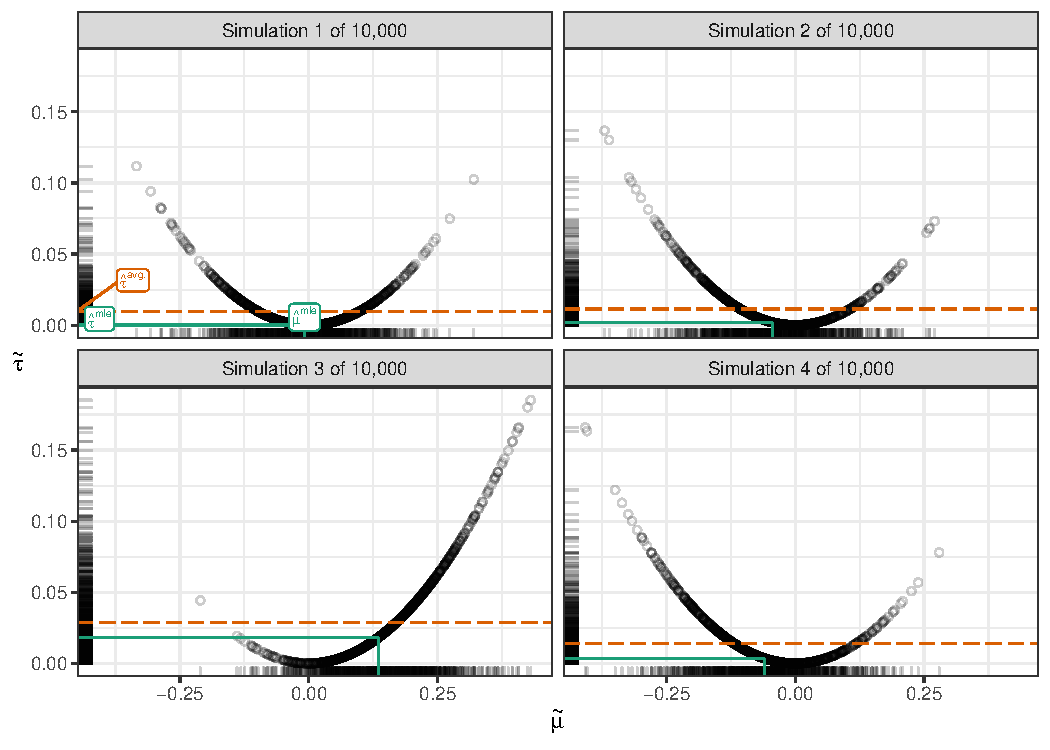
\includegraphics[width = 0.7\textwidth]{figs/intuition.pdf}\\
\vspace{.03in}
\caption{The first four Monte Carlo simulations of $\hat{mu}$. These four panels illustrate the relationship between $\hat{\tau}^\text{mle}$ and $\hat{\tau}^\text{avg}$ described by Lemma \ref{lem:direction} and Theorem \ref{thm:direction}.}\label{fig:samp}
\end{center}
\end{figure}

\begin{figure}[!h]
\begin{center}
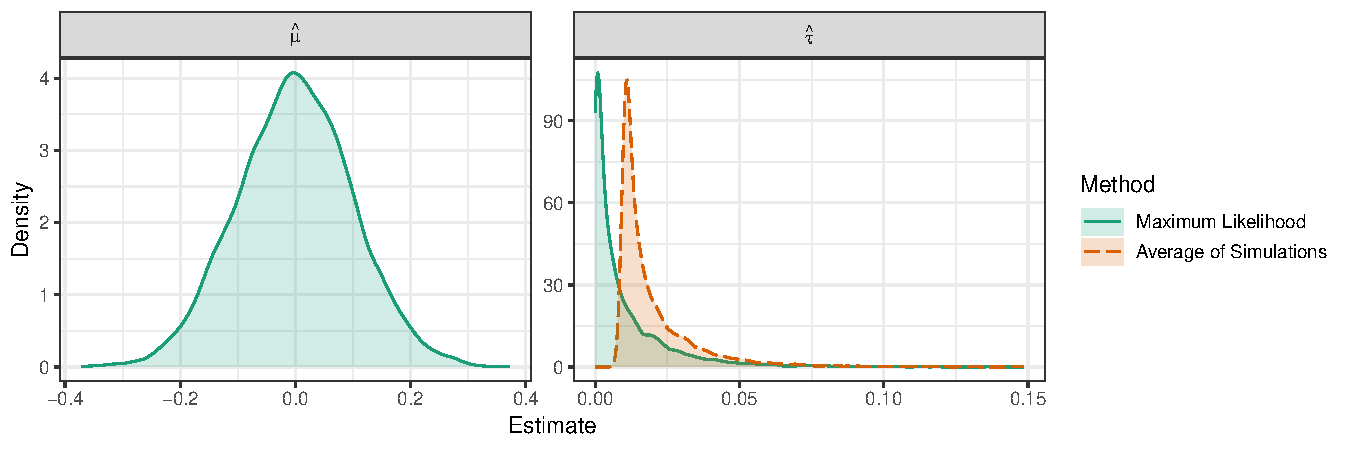
\includegraphics[width=0.8\textwidth]{figs/intuition-sampling.pdf}\\
\vspace{.03in}
\caption{The sampling distributions of $\hat{\beta}^\text{mle}$, $\hat{\tau}^\text{mle}$, and $\hat{\tau}^\text{avg}$.}\label{fig:int-samp}
\end{center}
\end{figure}

\subsection*{Using the Law of Iterated Expectations}

One can also develop the argument analytically via the law of iterated expectations. It helps to alter the notation slightly, making two implicit dependencies explicit. I explain each change below and use the alternate, more expansive notation only in this section.

The law of iterated expectations states that $\E_Y \left( \E_{X \mid Y}(X \mid Y) \right) = \E_X(X)$, where $X$ and $Y$ represent random variables.
The three expectations occur with respect to three different distributions: $\E_Y$ denotes the expectation with respect to the marginal distribution of $Y$, $\E_{X \mid Y}$ denotes the expectation with respect to the conditional distribution of $X \mid Y$, and $\E_X$ denotes the expectation with respect to the marginal distribution of $X$.

Outside of this section, the reader should understand that the distribution of $\tilde{\beta}$ depends on $\hat{\beta}^\text{mle}$ and could be written as $\tilde{\beta} \mid \hat{\beta}^\text{mle}$.
To remain consistent with previous work, especially \cite{KingTomzWittenberg2000} and \cite{Herron1999}, I use $\tilde{\beta}$ to represent $\tilde{\beta} \mid \hat{\beta}^\text{mle}$.
The definition of $\tilde{\beta}$ makes this usage clear.
In this section only, I use $\tilde{\beta} \mid \hat{\beta}^\text{mle}$ to represent the conditional distribution of $\tilde{\beta}$ and use $\tilde{\beta}$ to represent the \underline{un}conditional distribution of $\tilde{\beta}$.
Intuitively, one might imagine (1) generating a data set $y$, (2) estimating $\hat{\beta}^\text{mle}$, and (3) simulating $\tilde{\beta} \mid \hat{\beta}^\text{mle}$.
If I perform steps (1) and (2) just once, but step (3) repeatedly, I generate a sample from the conditional distribution $\tilde{\beta} \mid \hat{\beta}^\text{mle}$.
If I perform steps (1), (2), and (3) repeatedly, then I generate a sample from the \underline{un}conditional distribution $\tilde{\beta}$.
The unconditional distribution helps us understand the nature of the simulation-induced $\tau$-bias.

Applying the law of iterated expectations, I obtain $\E_{\tilde{\beta}} \left( \tilde{\beta} \right) = \E_{\hat{\beta}^\text{mle}}\left( \E_{\tilde{\beta} \mid \hat{\beta}^\text{mle}} (\tilde{\beta} \mid \hat{\beta}^\text{mle}) \right)$.
The three identities below connect the three key quantities from Theorem \ref{thm:direction} to three versions of $\E_{\hat{\beta}^\text{mle}}\left( \E_{\tilde{\beta} \mid \hat{\beta}^\text{mle}} (\tilde{\beta} \mid \hat{\beta}^\text{mle}) \right)$, with the transformation $\tau(\cdot)$ applied at different points.
\small
\begin{alignat}{2}
 \color{color1} \tikzmark{MarkA}\tau \left[ \normalcolor \E_{\hat{\beta}^\text{mle}}\left( \E_{\tilde{\beta} \mid \hat{\beta}^\text{mle}} \left( \tilde{\beta} \mid \hat{\beta}^\text{mle} \right) \right) \color{color1} \right] \normalcolor =&  \tau \left[ \E_{\tilde{\beta}} \left( \tilde{\beta} \right) \right] = \tau \left[\E\left( \hat{\beta}^\text{mle} \right) \right]\text{,} \label{eqn:true}\\
 \E_{\hat{\beta}^\text{mle}}\left( \color{color1} \tikzmark{MarkB}\tau\tikzmark{MarkC} \left[ \normalcolor \E_{\tilde{\beta} \mid \hat{\beta}^\text{mle}} \left( \tilde{\beta} \mid \hat{\beta}^\text{mle} \right) \color{color1} \right] \normalcolor \right)  =&  \E_{\hat{\beta}^\text{mle}} \left( \tau \left[\hat{\beta}^\text{mle} \right] \right) =  \E_{\hat{\beta}^\text{mle}} \left(\hat{\tau}^\text{mle} \right) \text{, and} \justif{\quad}{$\longleftarrow~$ Switch $\tau$ and an $\E$ once.} \label{eqn:mle}\\
\E_{\hat{\beta}^\text{mle}}\left( \E_{\tilde{\beta} \mid \hat{\beta}^\text{mle}} \left( \color{color1} \tikzmark{MarkD}\tau \left[ \normalcolor \tilde{\beta} \mid \hat{\beta}^\text{mle} \color{color1} \right] \normalcolor \right) \right)  =&
\E_{\tilde{\beta}} \left( \tau \left[\tilde{\beta} \right] \right)  =
\E_{\tilde{\beta}} \left(\hat{\tau}^\text{avg} \right) \text{.}\justif{\quad}{$\longleftarrow~$ Switch $\tau$ and an $\E$ again.}\label{eqn:avg}\DrawBox{red}{blue}
\end{alignat}
\normalsize

If I subtract Equation \ref{eqn:mle} from Equation \ref{eqn:true}, I obtain the transformation-induced $\tau$-bias in $\hat{\tau}^\text{mle}$ (see Equation \ref{eqn:ti-bias} for the definition of transformation-induced $\tau$-bias).
To move from Equation \ref{eqn:true} to Equation \ref{eqn:mle} I must swap $\tau(\cdot)$ with an expectation once.
This implies that, if $\tau(\cdot)$ is convex, Equation \ref{eqn:mle} must be greater than Equation \ref{eqn:true}.
This, in turn, implies that the bias is positive.

To obtain the $\tau$-bias in $\hat{\tau}^\text{avg}$ I must subtract Equation \ref{eqn:avg} from Equation \ref{eqn:true}.
But to move from Equation \ref{eqn:true} to Equation \ref{eqn:avg} I must swap $\tau(\cdot)$ with an expectation \emph{twice}.
Again, if $\tau(\cdot)$ is convex, then Equation \ref{eqn:avg} must be greater than Equation \ref{eqn:true}.
However, because one should expect $\hat{\beta}^\text{mle}$ and $\tilde{\beta} \mid \hat{\beta}^\text{mle}$ to have similar distributions, one should expect the additional swap to roughly double the bias in $\hat{\tau}^\text{avg}$ compared to $\hat{\tau}^\text{mle}$. This additional swap creates the additional, simulation-induced $\tau$-bias.

\subsection*{Using a Re-Analysis of Holland (2015)}

Holland (2015) presents a nuanced theory that describes the conditions under which politicians choose to enforce laws and supports the theoretical argument with a rich variety of evidence. In particular, it elaborates on the \textit{electoral} incentives of politicians to enforce laws. I borrow three Poisson regressions and hypotheses about a single explanatory variable to illustrate how the plug-in estimates can differ from the average-of-simulations estimate.

Holland writes: 
\begin{quote}
My first hypothesis is that enforcement operations drop off with the fraction of poor residents in an electoral district. So district poverty should be a negative and significant predictor of enforcement, but only in politically decentralized cities [Lima and Santiago]. Poverty should have no relationship with enforcement in politically centralized cities [Bogota] once one controls for the number of vendors.
\end{quote}

I use Holland's hypothesis and data to illustrate the behavior of the average-of-simulations and plug-in estimators. I refit Model 1 from Table 2 in \cite{Holland2015} for each city. I then use each model to compute the percent increase in the enforcement operations for each district in the city if the percent of the district in the lower class dropped by half. For example, in the Villa Maria El Triunfo district in Lima, 84\% of the district is in the lower class. If this dropped to 42\%, then the average-of-simulations estimate suggests that the number of enforcement operations would increase by about 284\% (from about 5 to about 20). The plug-in estimate, on the other hand, suggests an increase of 264\% (from about 5 to about 17). The plug-in estimate, then, is about 7\% smaller than the average-of-simulations estimate---a small, but noticeable shrinkage. 


Figure \ref{fig:holland} shows how the estimates change (usually shrink) for all districts when I switch from the average-of-simulations estimates to plug-in estimates. Table \ref{tab:top-5} presents the details for the labeled cases in Figure \ref{fig:holland}. In Bogota, the estimate shrinks by 11\% in Sante Fe and 16\% in Usme. In Lima, the estimate shrinks by 5\% in Chacalacayo and 7\% Villa Maria El Triunfo. The shrinkage is much larger in Santiago, where the standard errors for the coefficient estimates are much larger. The estimate shrinks by about 47\% in San Ramon and 53\% in La Pintana. The median shrinkage is 7\% in Bogota, 2\% in Lima, and 36\% in Santiago. For many districts in Santiago, the average-of-simulations estimate is about \textit{twice} the plugin estimate. These estimates clearly show that the average of simulations and the ML estimates can differ meaningfully in actual analyses.

\begin{figure}[h]
\begin{center}
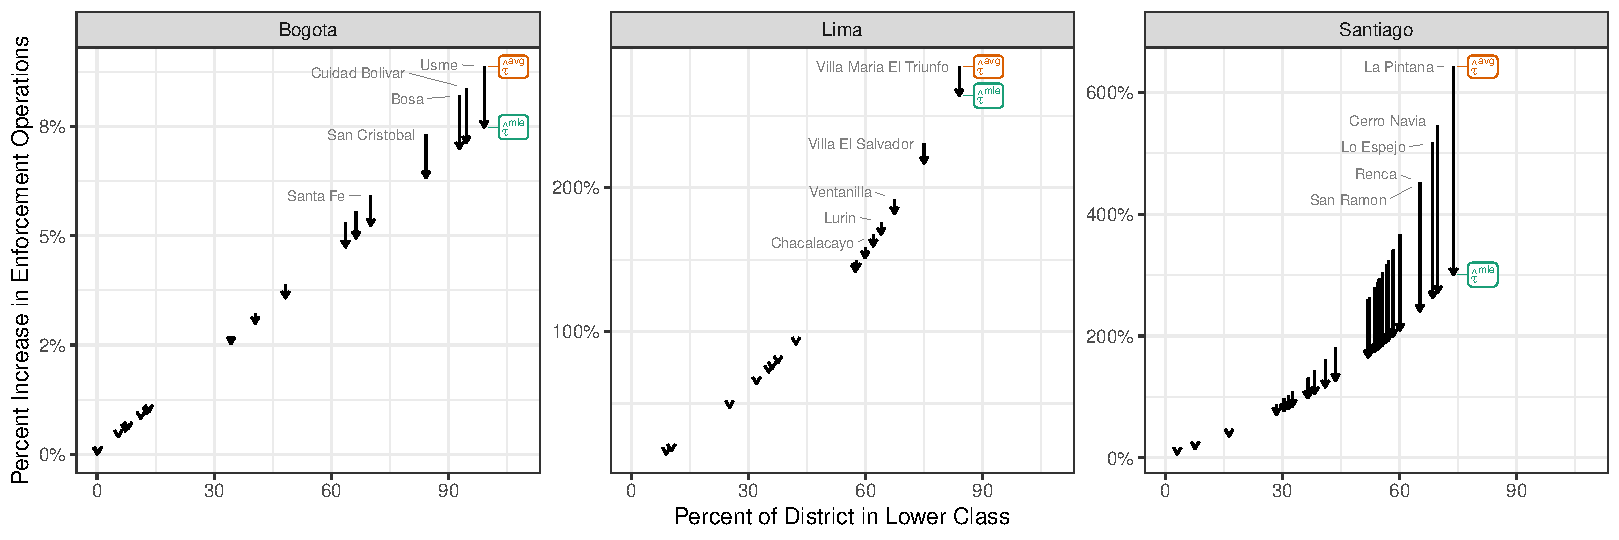
\includegraphics[width=\textwidth]{figs/holland.pdf}\\
\vspace{.1in}
\caption{This figure compares the average-of-simulations estimates with the plug-in estimates using three Poisson regression models from Holland (2015). The quantity of interest is the percent increase in the enforcement operations when the percent of a district in the lower class drops by half. The arrows show how the estimates change when I switch from the average-of-simulations to the plug-in estimate.}\label{fig:holland}
\end{center}
\end{figure}

\begin{table}[!h]

\caption{\label{tab:}\label{tab:top-5}This table presents the details for the districts labelled in Figure \ref{fig:holland}.}
\centering
\fontsize{8}{10}\selectfont
\begin{tabular}[t]{>{\bfseries}l>{\bfseries}lccccccc}
\toprule
\multicolumn{2}{c}{\bfseries  } & \multicolumn{3}{c}{\bfseries Average of Simulations} & \multicolumn{3}{c}{\bfseries ML Estimate} & \multicolumn{1}{c}{\bfseries  } \\
\cmidrule(l{2pt}r{2pt}){3-5} \cmidrule(l{2pt}r{2pt}){6-8}
\textbf{City} & \textbf{District} & \textbf{\% Change\textsuperscript{a}} & \textbf{From\textsuperscript{b}} & \textbf{To\textsuperscript{c}} & \textbf{\% Change} & \textbf{From} & \textbf{To} & \textbf{Shrinkage\textsuperscript{d}}\\
\midrule
 & Usme & 9\% & 5.5 & 5.8 & 7\% & 5.4 & 5.8 & 14\%\\

 & Cuidad Bolivar & 8\% & 6.1 & 6.4 & 7\% & 5.9 & 6.3 & 13\%\\

 & Bosa & 8\% & 7.1 & 7.4 & 7\% & 6.9 & 7.4 & 13\%\\

 & San Cristobal & 7\% & 12.7 & 13.4 & 6\% & 12.5 & 13.3 & 11\%\\

\multirow{-5}{*}{\raggedright\arraybackslash Bogota} & Santa Fe & 6\% & 27.3 & 28.9 & 5\% & 26.6 & 28.0 & 9\%\\
\cmidrule{1-9}
 & Villa Maria El Triunfo & 284\% & 5.2 & 19.4 & 264\% & 4.7 & 17.1 & 7\%\\

 & Villa El Salvador & 230\% & 7.2 & 23.3 & 217\% & 6.8 & 21.4 & 6\%\\

 & Ventanilla & 192\% & 8.4 & 23.4 & 182\% & 8.2 & 23.0 & 5\%\\

 & Lurin & 176\% & 6.9 & 17.4 & 168\% & 6.4 & 17.1 & 5\%\\

\multirow{-5}{*}{\raggedright\arraybackslash Lima} & Chacalacayo & 167\% & 6.7 & 16.4 & 159\% & 6.2 & 16.1 & 4\%\\
\cmidrule{1-9}
 & La Pintana & 642\% & 1.4 & 4.0 & 301\% & 0.8 & 3.4 & 53\%\\

 & Cerro Navia & 546\% & 1.5 & 4.3 & 272\% & 1.0 & 3.6 & 50\%\\

 & Lo Espejo & 517\% & 1.4 & 4.4 & 263\% & 1.0 & 3.5 & 49\%\\

 & Renca & 452\% & 1.3 & 4.1 & 241\% & 1.0 & 3.4 & 47\%\\

\multirow{-5}{*}{\raggedright\arraybackslash Santiago} & San Ramon & 452\% & 1.2 & 4.0 & 241\% & 1.0 & 3.3 & 47\%\\
\bottomrule
\multicolumn{9}{l}{\textsuperscript{a} Quantity of interest; percent change in enforcement operations when the percent in the lower class drops by half.}\\
\multicolumn{9}{l}{\textsuperscript{b} Enforcement operations when the percent in the lower class equals its observed value.}\\
\multicolumn{9}{l}{\textsuperscript{c} Enforcement operations when the percent in the lower class equals half its observed value.}\\
\multicolumn{9}{l}{\textsuperscript{d} Shrinkage in the quantity of interest due to switching from the average of simulations to the ML estimator.}\\
\end{tabular}
\end{table}

\section*{Conclusion}

Many social scientists turn to \cite{KingTomzWittenberg2000} for advice on interpreting, summarizing, and presenting empirical results. The authors improved empirical research by highlighting the importance of substantively meaningful quantities of interest. I agree with King and Zeng's (\citeyear{king2006dangers}) summary of the literature: “[w]hether such effects are calculated via analytical derivation or what is now the more common approach of statistical simulation, political scientists have made much progress in learning how to make sophisticated methods speak directly to their substantive research questions” (p. 132). 

Researchers estimate quantities of interest either by averaging simulated quantities of interest (e.g., CLARIFY in Stata, Zelig in R) or using the invariance property of maximum likelihood estimators (e.g., margins in Stata and R). In practice, researchers' choice between these two estimators seems idiosyncratic rather than principled, depending on their preferred software package rather than any statistical criteria. The methodological literature recommends both, but has not distinguished or compared the two approaches to estimating quantities of interest.

When researchers use the average of simulations (King, Tomz, and Wittenberg 2000) to estimate quantities of interest, they replicate the logic of transformation-induced bias (Rainey 2017) and add simulation-induced bias to the estimates. This additional bias is roughly the same magnitude and direction as transformation-induced bias and occurs \textit{in addition to} transformation-induced bias. While the additional bias is usually small relative to the standard error, methodologists should not recommend methods that add unnecessary bias to point estimates. Instead, we should recommend methods that better adhere to the usual evaluative standards. Even if we recommend using simulation to estimate standard errors, we should not recommend averaging simulations to obtain the point estimate. Instead, researchers should directly transform maximum likelihood estimates of coefficients to obtain maximum likelihood estimates of the quantities of interest. The resulting point estimates inherit the desirable properties of maximum likelihood estimators and avoid unnecessary simulation-induced bias.

\singlespace
%\clearpage
\small
\bibliographystyle{apsr_fs}
\bibliography{bibliography}
\end{document}
